\documentclass[12pt]{article}
\usepackage{indentfirst, setspace, tikz, xcolor}	
\usepackage[margin=1in]{geometry}
\usetikzlibrary{decorations.pathreplacing, calc}

\definecolor{lightBlue}{RGB}{173,221,237}


\begin{document}

\setstretch{1.3}

	Abnormalities in rainfall in Western Australia and New Zealand have reduced the harvesting output of avocados by 30\%. Concurrently, marketing and health campaigns proclaiming the benefits of avocados have increased demand. Consequently, avocado prices have hit a record high. \\
	
	Demand refers to the various quantities of a good that consumers are willing and able to buy at various prices during a period of time. Similarly, supply refers to the various quantities of a good that producers are willing and able to supply at various prices during a period of time. Note, though, that quantity demanded and quantity supplied differ from demand and supply because they refer to a particular quantity at a particular price. \\
	
	\begin{center}

\ \ \ \ \ Figure 1. The Market for Avocados

\vspace{0.5\baselineskip}

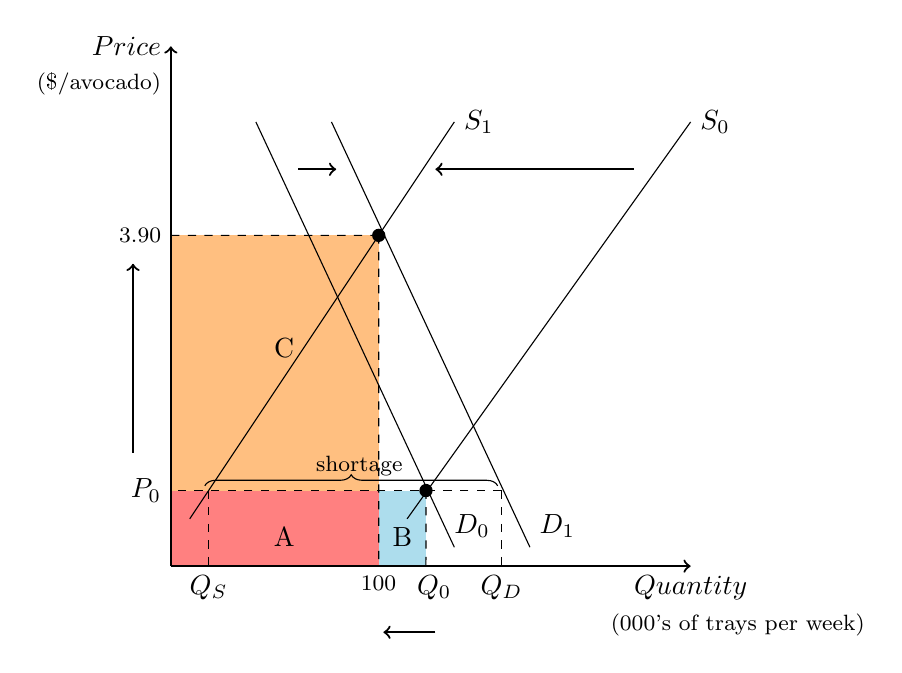
\begin{tikzpicture}[scale= 1.2]

% Define coordinates.

	%axes

	\coordinate (origin) at (0,0);
	\coordinate [label= left:$Price$] (P) at (0, 5.5);
	\coordinate [label= below:$Quantity$] (Q) at (5.5, 0);
	
	%demand curve 1
	\coordinate (demandTail) at (1.7, 4.7);
	\coordinate (D) at (3.8, 0.2);
	
	%demand curve 0
	\coordinate (demandTail0) at (0.9, 4.7);
	\coordinate (D0) at (3, 0.2);
		
	%supply curve 1 
	\coordinate (supplyTail1) at (0.2, 0.5);
	\coordinate [label = right:$S_1$] (S) at (3, 4.7);
	
	%supply curve 0
	\coordinate (supplyTail0) at (2.5, 0.5);
	\coordinate [label= right:$S_0$] (S0) at (5.5, 4.7);
	
	%Equilibria 
	\coordinate (E0) at (2.7, 0.8);	
	\coordinate (E1) at (2.2, 3.5);
	
%colour rev boxes
	\fill [fill=lightBlue] (origin) rectangle (E0);
	\fill [fill=orange!50] (origin) rectangle (E1);
	\fill [fill=red!50] (origin) rectangle (2.2, 0.8);
	 
% Draw axes.

	\draw[thick, ->] (origin) -- (P);
	\draw[thick, ->] (origin) -- (Q);  
	
% Draw lines.

	\draw (demandTail0) -- (D0)node[above right, xshift=-3.5pt] {$D_0$};		
	\draw (demandTail) -- (D)node[above right] {$D_1$};
	\draw (supplyTail1) -- (S);
	\draw (supplyTail0) -- (S0);
	
	\draw[dashed] (E0) -- (2.7, 0) node[below, xshift=3pt] {$Q_0$};
	\draw[dashed] (3.5, 0.8) -- (0, 0.8) node[left] {$P_0$};
	
	\draw[dashed] (E1) -- (2.2, 0) node[below, xshift=-0.1pt] {\footnotesize $100$};
	\draw[dashed] (E1) -- (0, 3.5) node[left] {\footnotesize $3.90$};
	\draw[dashed] (3.5, 0.8) -- (3.5, 0) node[below] {$Q_D$};
	\draw[dashed] (0.4, 0.8) -- (0.4, 0) node[below] {$Q_S$};
	
	\draw[thick, ->](4.9, 4.2) -- (2.8, 4.2);
	\draw[thick, ->](1.35, 4.2) -- (1.75, 4.2);
	
% Draw area labels.

	\draw (1.2, 0.1) node[above]{A};
	\draw (2.45, 0.1) node[above]{B};
	\draw (1.2, 2.1) node[above]{C};
	
% Draw label arrows.

	\draw[thick, ->] (-0.4, 1.2) -- (-0.4, 3.2); 
	\draw[thick, ->] (2.8, -0.7) -- (2.25, -0.7);

% Draw equlibria.

	\fill[black] (E0) circle (2pt);
	\fill[black] (E1) circle (2pt);
	
		\draw [decorate, decoration ={brace,amplitude=4pt},xshift=-4pt,yshift=0pt] ($(0.4, 0.8) + (0.1, 0.05)$) -- ($(3.5, 0.8) + (0.1, 0.05)$) node [above, xshift=-50pt] {\footnotesize shortage}; 
		
		\draw (6, -0.4) node [below]{\footnotesize (000's of trays per week)};
		\draw (0, 5.1) node [left]{\footnotesize (\$/avocado)};

\end{tikzpicture}
\end{center} 
	
	When demand and supply move in opposition, equilibrium quantity is indeterminate. In recent times quantity supplied of avocados has been declining from some quantity, $Q_0$, to around 100 000 trays per week. We can deduce that the magnitude of the shift left of the supply curve|in this case from $S_0$ to $S_1$|was greater than that of the shift right of the demand curve from $D_0$ to $D_1$. As illustrated in Figure 1, the outcome of these shifts is a substantial increase in price from $P_1$ to $\$3.90$ per avocado. %should this price be in price per tray ($75)? \\
	
	In the short run, a price of $P_0$ effects a disparity between quantity supplied, $Q_S$ and quantity demanded, $Q_D$. The positive difference between $Q_D$ and $Q_S$, is the shortage, the excess of quantity demanded over quantity supplied, at $P_0$. This puts upward pressure on equilibrium price, because consumers are willing and able to pay more than it for avocados. They will likely try to outbid each other, and in the long run, equilibrium price will increase. \\
	
	 Avocado has a relatively low price elasticity in demand (PED, $\frac{\% \Delta Q_D}{\% \Delta P_x}$), which makes it price inelastic in demand. PED gauges how responsive quantity demanded is to a given change in price. Avocados' uniqueness does not allow it to be easily replaced, so because of the lack of alternatives, consumers will not react significantly to changes in price. Thus, in the case of avocados, a change in quantity demanded will be proportionately lesser than a given change in price. \\
	 
	Total revenue (TR), a firms' total earnings from a specified level of sales within a specified period of time, is calculated as quantity traded $\times$ unit price. The coloured rectangles in Figure 1 represent the revenues earned by producers. Area $A + C$, the revenue after the changes in demand and supply, is visually larger than area $A + B$, the revenue before the changes in demand and supply|TR increases, which is good news for most suppliers who can now enjoy a more lucrative production of avocados. \\
	
	Alternatively, consumers have to pay more for the avocados they want. Further, the supply of avocados is dwindling, so price will continue to rise. Thus, consumers get the short end of the stick.	
	
		\begin{center}

\ \ \ \ \ Figure 2. The Future of the Market for Avocados

\vspace{0.5\baselineskip}

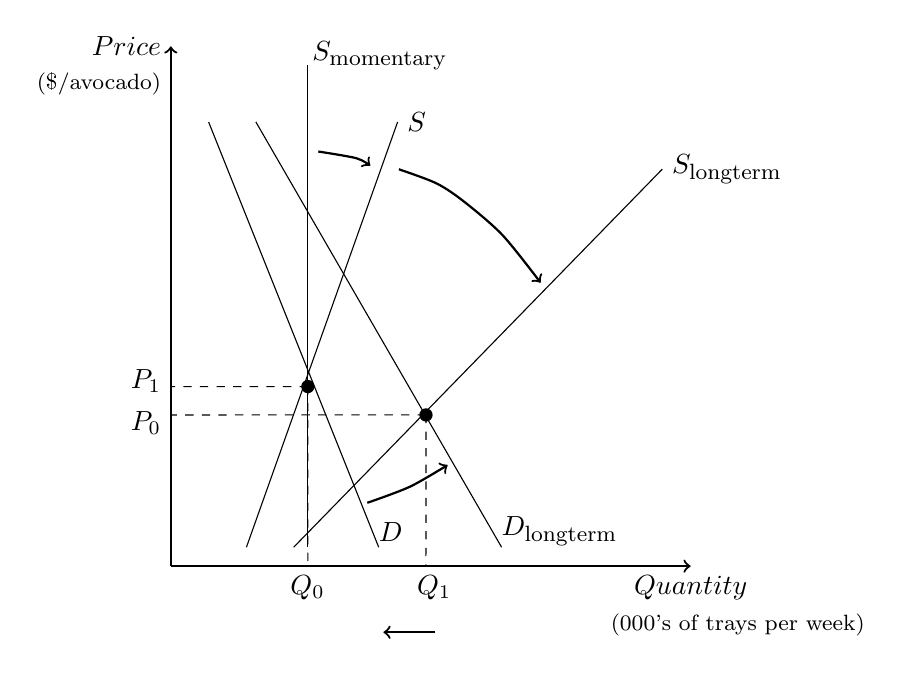
\begin{tikzpicture}[scale= 1.2]

% Define coordinates.

	%axes

	\coordinate (origin) at (0,0);
	\coordinate [label= left:$Price$] (P) at (0, 5.5);
	\coordinate [label= below:$Quantity$] (Q) at (5.5, 0);
	
	%demand curve 1
	\coordinate (demandTail) at (0.9, 4.7);
	\coordinate (D) at (3.5, 0.2);
	
	%demand curve 0
	\coordinate (demandTail0) at (0.4, 4.7);
	\coordinate (D0) at (2.2, 0.2);
		
	%supply curve 0 
	\coordinate (supplyTail0) at (0.8, 0.2);
	\coordinate [label = right:$S$] (S0) at (2.4, 4.7);
	
	%supply curve 1
	\coordinate (supplyTail) at (1.3, 0.2);
	\coordinate [label= right:$S_{\footnotesize \textrm{longterm}}$] (S) at (5.2, 4.2);
	
	%momentary supply curve
	\coordinate (sm1) at (1.45, 0.2);
	\coordinate (sm2) at (1.45, 5.3);
	
	%Equilibria 
	\coordinate (E0) at (2.7, 1.6);	
	\coordinate (E1) at (1.45, 1.9);
	
%colour rev boxes
	%\fill [fill=lightBlue] (origin) rectangle (E0);
	%\fill [fill=orange!50] (origin) rectangle (E1);
	%\fill [fill=red!50] (origin) rectangle (2.2, 0.8);
	 
% Draw axes.

	\draw[thick, ->] (origin) -- (P);
	\draw[thick, ->] (origin) -- (Q);  
	
% Draw lines.

	\draw (demandTail0) -- (D0)node[above right, xshift=-3.5pt, yshift=-1.5pt] {$D$};		
	\draw (demandTail) -- (D)node[above right, xshift=-3.5pt, yshift=-3pt] {$D_{      \footnotesize \textrm{longterm}}$};
	\draw (supplyTail) -- (S);
	\draw (supplyTail0) -- (S0);
	\draw (sm1) -- (sm2) node[above, xshift=26pt, yshift=-5pt]{$S_{ \footnotesize \textrm{momentary}}$};
	
	\draw[dashed] (E0) -- (2.7, 0) node[below, xshift=3pt] {$Q_1$};
	\draw[dashed] (E0) -- (0, 1.6) node[left, yshift=-3pt] {$P_0$};
	
	\draw[dashed] (E1) -- (1.45, 0) node[below, xshift=-0.1pt] {$Q_0$};
	\draw[dashed] (E1) -- (0, 1.9) node[left, yshift=2pt] {$P_1$};

	

	\draw[thick, ->, xshift=6pt, yshift=2.5pt] plot [smooth] coordinates {(1.35, 4.3)(1.75, 4.23)(1.9, 4.15)};
	
	\draw[thick, ->, xshift=-11pt] plot [smooth] coordinates {(2.8, 4.2)(3.2, 4.05)(3.5, 3.85)(3.9, 3.5)(4.3, 3)};
	
	\draw[thick, ->, xshift=-2pt, yshift=2pt] plot [smooth] coordinates {(2.15, 0.6)(2.6, 0.77)(3, 1)};

	
% Draw area labels.

	%\draw (1.2, 0.1) node[above]{A};
	%\draw (2.45, 0.1) node[above]{B};
	%\draw (1.2, 2.1) node[above]{C};
	
% Draw label arrows.

	%\draw[thick, ->] (-0.4, 1.2) -- (-0.4, 3.2); 
	\draw[thick, ->] (2.8, -0.7) -- (2.25, -0.7);

% Draw equlibria.

	\fill[black] (E0) circle (2pt);
	\fill[black] (E1) circle (2pt);
	
		
		\draw (6, -0.4) node [below]{\footnotesize (000's of trays per week)};
		\draw (0, 5.1) node [left]{\footnotesize (\$/avocado)};

\end{tikzpicture}
\end{center} 
	
	Despite avocado's uniqueness, in the long term, consumers will have had the time to search for possible alternative for avocados. For example, consumers might think that avocados too expensive and decide to start purchasing chayote squashes instead. However, this is not to say that demand itself will remain static (it historically has and is projected to do so too), only that avocados will become more price elastic in demand with time. These changes are illustrated as the shift and rotation of $D$ to $D_\textrm{longterm}$ in Figure 2. \\
	
	The momentary supply of avocados is fixed at a price elasticity in supply (PES, ${\frac{\% \Delta Q_S}{\% \Delta P_x}}$) of 0 by planting decisions made months or years before harvest. Momentary supply in the immediate short term is when the only amount available of a good is that which is already in the market. Given a change in price in the immediate short term, producers will not have the time to react and change their production of avocados. However, if we increase the time frame that we analyze, suppliers then have time to adjust production levels resulting in an increase in PES. Also, within the next few years, supply is expected to be bolstered by extra orchards that are currently growing. These changes are illustrated as the shifts and rotations from $S_\textrm{momentary}$ to $S$ to $S_\textrm{longterm}$. \\
	
	Since the relative magnitudes of these shifts are unknown, price is indeterminate. However, with that information we could determine whether the change in supply is greater than the change in demand, whether prices fall, and whether consumers or producers are winners in that situation. Figure 2 is a scenario in which price falls ($P_0$ to $P_1$) and consumers win.
\end{document} \\
